\fancyhead[L]{\textbf{\textsf{MỤC 1.2}}\quad Mô hình toán học: Danh mục các hàm số cơ bản}
\fancyhead[R]{\textsf{31}}

\noindent
\begin{minipage}[t]{0.26\textwidth}
    \vspace{0pt}
    \centering
    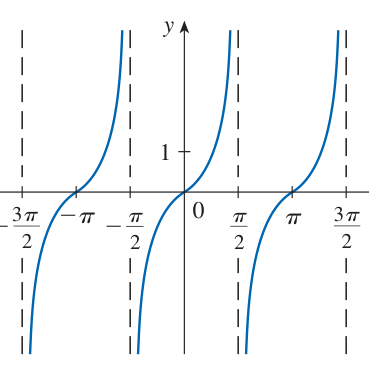
\includegraphics[width=\linewidth]{images/p0066_fig1.png}
    \vspace{-0.5em}
    \begin{flushleft}
        \textbf{\textsf{HÌNH 20}}\\
        $y = \tan x$
    \end{flushleft}

    \vspace{3.44em}
    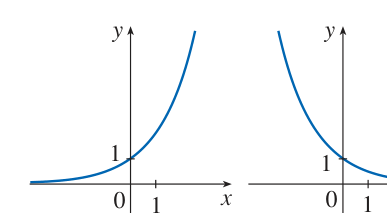
\includegraphics[width=\linewidth]{images/p0066_fig2.png}
    \vspace{-0.5em}
    \begin{flushleft}
        \textbf{\textsf{HÌNH 21}}
    \end{flushleft}

    \vspace{5.33em}
    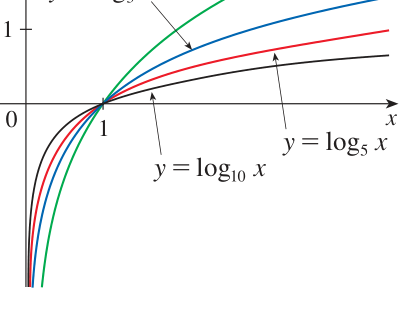
\includegraphics[width=\linewidth]{images/p0066_fig3.png}
    \vspace{-0.5em}
    \begin{flushleft}
        \textbf{\textsf{HÌNH 22}}
    \end{flushleft}
\end{minipage}%
\hfill
\begin{minipage}[t]{0.71\textwidth}
    \vspace{0pt}
    \noindent\textbf{\textsf{\color{stewartcyan}VÍ DỤ 5}}\quad Tìm tập xác định của hàm số $f(x) = \dfrac{1}{1 - 2\cos x}$.

    \vspace{0.33em}
    \noindent\textbf{\textsf{\color{stewartcyan}LỜI GIẢI}}\quad Hàm số này xác định với mọi giá trị của $x$ ngoại trừ các giá trị làm cho mẫu số bằng $0$. Ta có
    \[
    1 - 2\cos x = 0 \iff \cos x = \frac{1}{2} \iff x = \frac{\pi}{3} + 2n\pi \quad\text{hoặc}\quad x = \frac{5\pi}{3} + 2n\pi
    \]
    trong đó $n$ là một số nguyên bất kỳ (do hàm cosin tuần hoàn với chu kỳ $2\pi$). Vì vậy, tập xác định của $f$ là tập hợp tất cả các số thực ngoại trừ các số nêu trên.\hfill{\color{stewartcyan}$\blacksquare$}

    \vspace{0.66em}
    Hàm tang có liên hệ với hàm sin và cosin theo công thức
    \[
    \tan x = \frac{\sin x}{\cos x}
    \]
    và đồ thị của nó được cho trong Hình 20. Hàm số không xác định bất cứ khi nào $\cos x = 0$, tức là khi $x = \pm\pi/2, \pm 3\pi/2, \dots$. Tập giá trị của nó là $(-\infty, \infty)$. Chú ý rằng hàm tang có chu kỳ là $\pi$:
    \[
    \tan(x + \pi) = \tan x \quad\text{với mọi } x
    \]

    Ba hàm số lượng giác còn lại (cosecant, secant và cotangent) lần lượt là các hàm nghịch đảo của hàm sin, cosin và tang. Đồ thị của chúng được trình bày trong Phụ lục D.

    \vspace{0.66em}
    \noindent{\color{stewartcyan}\rule{1.2ex}{1.2ex}}\hspace{0.5em}\textbf{\textsf{Hàm số mũ}}
    \nopagebreak

    \vspace{0.25em}
    \noindent\textbf{Hàm số mũ} là các hàm số có dạng $f(x) = b^x$, trong đó cơ số $b$ là một hằng số dương. Đồ thị của $y = 2^x$ và $y = (0.5)^x$ được biểu diễn trong Hình 21. Trong cả hai trường hợp, tập xác định là $(-\infty, \infty)$ và tập giá trị là $(0, \infty)$.

    Hàm số mũ sẽ được nghiên cứu chi tiết trong Mục 1.4, và chúng ta sẽ thấy rằng chúng rất hữu ích trong việc mô hình hóa nhiều hiện tượng tự nhiên, chẳng hạn như sự tăng trưởng dân số (nếu $b > 1$) hoặc sự suy giảm (nếu $b < 1$).

    \vspace{0.66em}
    \noindent{\color{stewartcyan}\rule{1.2ex}{1.2ex}}\hspace{0.5em}\textbf{\textsf{Hàm số logarit}}
    \nopagebreak

    \vspace{0.25em}
    \noindent\textbf{Hàm số logarit} $f(x) = \log_b x$, với cơ số $b$ là một hằng số dương, là các hàm ngược của hàm số mũ. Chúng sẽ được nghiên cứu trong Mục 1.5. Hình 22 minh họa đồ thị của bốn hàm số logarit với các cơ số khác nhau. Trong mỗi trường hợp, tập xác định là $(0, \infty)$, tập giá trị là $(-\infty, \infty)$, và hàm số tăng chậm khi $x > 1$.

    \vspace{0.66em}
    \noindent\textbf{\textsf{\color{stewartcyan}VÍ DỤ 6}}\quad Hãy phân loại các hàm số sau đây theo một trong các loại hàm số mà chúng ta đã thảo luận.
    \begin{tasks}[column-sep=1em](4)
        \task $f(x) = 5^x$
        \task $g(x) = x^5$
        \task $h(x) = \dfrac{1 + x}{1 - \sqrt{x}}$
        \task $u(t) = 1 - t + 5t^4$
    \end{tasks}

    \vspace{0.33em}
    \noindent\textbf{\textsf{\color{stewartcyan}LỜI GIẢI}}
    \begin{enumerate}[(a)]
        \item $f(x) = 5^x$ là một hàm số mũ. (Biến số $x$ đóng vai trò là số mũ.)
        \item $g(x) = x^5$ là một hàm lũy thừa. (Biến số $x$ đóng vai trò là cơ số.) Chúng ta cũng có thể coi nó là một đa thức bậc 5.
        \item $h(x) = \dfrac{1 + x}{1 - \sqrt{x}}$ là một hàm đại số. (Nó không phải là một hàm phân thức hữu tỉ vì mẫu số không phải là một đa thức.)
        \item $u(t) = 1 - t + 5t^4$ là một đa thức bậc 4.
    \end{enumerate}
    \vspace{-1.2em}\hfill{\color{stewartcyan}$\blacksquare$}

    \vspace{0.66em}
    Bảng 3 (ở trang tiếp theo) tóm tắt đồ thị của một số họ hàm số cơ bản thường xuyên được sử dụng xuyên suốt cuốn sách này.
\end{minipage}